% CVPR 2022 Paper Template
% based on the CVPR template provided by Ming-Ming Cheng (https://github.com/MCG-NKU/CVPR_Template)
% modified and extended by Stefan Roth (stefan.roth@NOSPAMtu-darmstadt.de)

\documentclass[10pt,twocolumn,letterpaper]{article}

%%%%%%%%% PAPER TYPE  - PLEASE UPDATE FOR FINAL VERSION
\usepackage[review]{cvpr}      % To produce the REVIEW version
% \usepackage{cvpr}              % To produce the CAMERA-READY version
%\usepackage[pagenumbers]{cvpr} % To force page numbers, e.g. for an arXiv version

% Include other packages here, before hyperref.
\usepackage{graphicx}
\usepackage{amsmath}
\usepackage{amssymb}
\usepackage{booktabs}
\usepackage{rotating}
\usepackage{caption}
\usepackage{subcaption}

% It is strongly recommended to use hyperref, especially for the review version.
% hyperref with option pagebackref eases the reviewers' job.
% Please disable hyperref *only* if you encounter grave issues, e.g. with the
% file validation for the camera-ready version.
%
% If you comment hyperref and then uncomment it, you should delete
% ReviewTempalte.aux before re-running LaTeX.
% (Or just hit 'q' on the first LaTeX run, let it finish, and you
%  should be clear).
\usepackage[pagebackref,breaklinks,colorlinks]{hyperref}


% Support for easy cross-referencing
\usepackage[capitalize]{cleveref}
\crefname{section}{Sec.}{Secs.}
\Crefname{section}{Section}{Sections}
\Crefname{table}{Table}{Tables}
\crefname{table}{Tab.}{Tabs.}


%%%%%%%%% PAPER ID  - PLEASE UPDATE
\def\cvprPaperID{*****} % *** Enter the CVPR Paper ID here
\def\confName{CVPR}
\def\confYear{2022}

\newcommand{\AJ}[1]{{\color{red}{[Andrej: #1]}}}

\begin{document}

%%%%%%%%% TITLE - PLEASE UPDATE
\title{Self-Supervised Transfer Learning From 2D Images to 3D Point Clouds}

\author{Andrej Janda\\
University of Toronto Institute for Aerospace Studies\\
Institution1 address\\
{\tt\small andrej.janda@robotics.utias.utoronto.ca}
% For a paper whose authors are all at the same institution,
% omit the following lines up until the closing ``}''.
% Additional authors and addresses can be added with ``\and'',
% just like the second author.
% To save space, use either the email address or home page, not both
\and
Jonathan Kelly\\
University of Toronto Institute for Aerospace Studies\\
First line of institution2 address\\
{\tt\small jonathan.kelly@robotics.utias.utoronto.ca}
}
\maketitle

%%%%%%%%% ABSTRACT
\begin{abstract}
    We show that previous work \cite{xie2020pointcontrast} on self-supervised contrastive learning of 3D point clouds relies on extrapolating points in the scene and not from learning noise as was claimed in the original paper. We then investigate if using 2D pre-trained features transfered to 3D can do as well as fully supervised learning.
\end{abstract}

%%%%%%%%% BODY TEXT
\section{Introduction}
\label{sec:intro}

% Write topic sentences and go from there
Segmentation of indoor 3D scenes has the potential to allow robots to navigate and interact with complicated industrial environments, such as warehouses and production facilities. Although robots already play a limited role in these facilities, understanding their surroundings would give them much greater autonomy. For instance, through segmentation, an accurate up-to-date digital twin of a physical area can be maintained for the purposes of inventory management, item retrieval, and item routing. Advances in segmentation of 3D point clouds \cite{choy20194d} has made this closer to reality.

Alternatively, segmentation of 2D images has come a long way. But it does not give us information about the 3D world and so we are left with projecting these predictions into 3D. This was the approach taken by \cite{} but has recently been overtaken by methods operating purely in 3D.

In contrast to 2D images which are bountiful, easy to collect and annotate, 3D scenes are hard to collect, not very abundant and notoriously hard to annotate. Collecting 3D scenes requires a user to physically scan different environments with complicated sensors (\eg stereo cameras, Lidar) and estimate the mapping between measurements to generate a completed scene. Since not everyone has access to these sensors, they cannot be easily scrapped off of the web. Still, the hardest component is annotation which requires users to manipulate 3D scenes and select only those points that belong to a particular object. This motivates us to look for ways of avoiding the annotation process and leverage un-labeled 3D data instead.

It is common practice in image tasks to use a model that was pre-trained in a supervised way on a larger but different dataset. However, recent works have been exploring the use of self-supervised objectives without labels in 2D image classification and found that they can greatly improve downstream accuracy, even matching fully supervised training \cite{}.

Recently, works such as \cite{xie2020pointcontrast} have shown that these methods also work with 3D data. Similar to 2D methods they use a contrastive loss objective where the goal is to learn distinguishing features between different datapoints and their respective augmentations.

These algorithms work exclusively with point clouds but throw away the corresponding images of the scene which provide a rich and dense source in extra information that can be used in downstream training. This paper investigates how this extra data modality can be leveraged. Additionally, it investigates the properties of an existing 3D pre-training algorithm.

This paper has the following contributions.

\begin{itemize}
    \item Demonstrates that previous work in 3D \cite{xie2020pointcontrast} works by learning to extrapolate 3D scenes. When purely learning improved features on fully-overlapping regions the performance gain disapears.
    \item Provide a 2D feature extractor and pre-training algorithm. Demonstrate that these features can improve 2D segmentation.
    \item Transfer learned 2D features onto a 3D model
\end{itemize}

\section{Related Work}
\label{sec:relatedWork}


\textbf{Sparse 3D convolutions.} Talk about submanifold networks, Minkowski Engine, etc

\textbf{Contrastive Learning.} Talk about SimCLR, BOYL, etc. Then talk about PointContrast.

\textbf{Knowledge Distilation} Need to read up on this


\section{Self-Supervised Contrastive learning}
\label{sec:contrastiveLearning}

The goal of self-supervised transfer learning is to learn from unlabeled data using a self-supervised objective which in turn initializes a model's backbone. The initialization is meant to improve performance of downstream tasks. Specifically, contrastive learning uses an objective function that encourages the outputs of a model on similar datapoints to be close together while keeping those of dissimilar datapoints to be far apart, in some metric space.

Defining what datapoints are similar and dissimilar depends on the pretext task. Image colorization for example defines color pixels and their grayscale equivalent as similar and all other pixels as dissimilar. In this work, we adopt the instance discrimination task as in \cite{} whereby each input individually is taken to belong to its own class.

We follow the formulation from \cite{le-khac_contrastive_2020}. Given a sampled point $\mathbf{x}$, positive points are sampled according to a positive distribution $\mathbf{x}^{+} \sim p^{+}( \cdot | \mathbf{x})$ which is commonly defined as a set of transformations $t$ of the original point. Often, positive pairs are derived by applying two different augmentations to the input point, $\mathbf{x}^{+} = t_{1}(\mathbf{x}), \, \mathbf{x} = t_{2}(\mathbf{x})$. Conversely, negative points are sampled according to $\mathbf{x}^{-} \sim p^{-}( \cdot | \mathbf{x})$ which in the context of an instance discriminative task means that they are taken as any other point not derived from the input point, regardless of its augmentation.

This point is fed through an encoder $e()$ to get feature $\mathbf{v} = e(\mathbf{x}), \mathbf{v} \in \mathbb{R}^d$. This encoder is the backbone of the model we are trying to initialize. The embedding is subsequently passed through a decoder $h()$ to generate a normalized latent representation $\mathbf{z}=h(\mathbf{v})$ with $\{\mathbf{z} \, | \, \mathbf{z} \in \mathbb{R}^{m}, \lVert \mathbf{z} \lVert^{2} = 1\}$  and where $m \leq d$. Once pretrained, only the encoder parameters are retained as the initialized backbone.

As for the objective function, we adopt an InfoNCE (Info Noise Contrastive Estimation) loss. It computes a negative log probability of an embedding's similarity to the embedding of its corresponding positive sample. This is conditioned by the similarity of that embedding to all the negative embeddings. It is defined as:
\begin{equation}
    \mathcal{L}_{i} = -\log \frac{\exp(\mathbf{z}_{i} \cdot \mathbf{z}^{+}_{i} / \tau)}{\exp(\mathbf{z}_{i} \cdot \mathbf{z}^{+}_{i} / \tau) + \sum^{K}_{j}\exp(\mathbf{z}_{i} \cdot \mathbf{z}^{-}_{j} / \tau)}
    \label{eq:contrastive_loss}
\end{equation}

Where $\tau \in (0,1]$ and represents the temperature parameter that controls the smoothness of the latent representations. $K$ is a hyperparameter that represents the number of negative embeddings to sample. Similarity between features is computed as the dot product.

\section{Feature Extraction}
\label{sec:featureExtraction}

This section goes through the types of backbones used as well as how features are extracted from 2D images and transferred to a 3D model.

\AJ{Need a picture depicting the pipeline}

\subsection{Extracting 2D features}
\label{sec:method:features2d}

We follow the ResUNet architecture from Godard \etal \cite{godard2019Digging}, which proved hugely successful in self-supervised monocular depth estimation. Its backbone consists of a ResNet34 with weights that were pretrained on ImageNet. Instead of estimating depth however, our decoder computes a 16 dimensional feature vector for each pixel in the input image.

Images are selected from the desired pre-training dataset. Positive samples are generated by randomly cropping the image, and then applying the following transformations: random horizontal flip, random gray-scale, gaussian blur and color jitter.

Only pixels found in the overlap of the two crops are used in the objective function. Corresponding pixels are taken as positive samples while all others, including from other images in a batch are taken as negatives.

This is then passed through the loss function described in \ref{eq:contrastive_loss}.

\AJ{Add figure of what your feature extractor looks like}

\AJ{Need to review how I do this in the code, I think I use a projector left over from BYOL}

\subsection{Feature projection}
\label{sec:featureProjection}

Here we leverage that images are a projection of 3D space. We assume that from a given viewpoint we have both an image as well as a depth or range scan, which is often the case when capturing raw data. Unlike in \cite{xie2020pointcontrast}, we don't require a pose linking adjacent frames making our method applicable to more use cases.

The two modalities can be mapped by projecting the point cloud into the color image using a standard pinhole camera model as defined below \cite{?}:

\begin{equation}
    \begin{bmatrix}
        u \\
        v \\
        1
    \end{bmatrix} = \frac{1}{z}
    \begin{bmatrix}
        f_u & 0   & c_u & 0 \\
        0   & f_v & c_v & 0 \\
        0   & 0   & 0   & 1 \\
    \end{bmatrix}
    \begin{bmatrix}
        x \\
        y \\
        z \\
        1 \\
    \end{bmatrix}
    \label{eq:pinhole}
\end{equation}

\AJ{Is this equation necessary or is this considered common knowledge}

Where $f$ represents focal length, $c$ the center offset, $u,v$ the pixels of an image and $x,y,z$ the 3D coordinates of the input point.

In the case of stereo cameras, this step is unnecessary as the mapping comes directly from the depth image. Note that its important to have the viewpoints of the 2D and 3D sensors be as close together as possible. This is exactly true for stereo cameras, but not guaranteed when using different sensors for each modality. Its important because occluded points can falsely be mapped to a pixel even though they are not directly visible in the image. Note also that using scans as opposed to any point cloud is also a limitation of \cite{xie2020pointcontrast}.

If the viewpoints are slightly off or the point cloud is a reconstruction from multiple scans, hidden points can be removed using the algorithm from Katz \etal \cite{katz2007Direct}.

After passing in the image through the model, the output is a scaled version of the original image. To complete the mapping, we can either take the feature with the closest feature pixel or interpolate the features using bi-linear interpolation. We will show an analysis of these two methods in section \ref{sec:results}

\AJ{Do I need to give the equation for Bi-linear interpolation or is this also considered basic knowledge}

\subsection{Feature Transfer}
\label{sec:featureTransfer}

Our last step, after generating 2D features and mapping them to 3D points is to train our 3D model to emulate our pre-trained features. We accomplish this using the same contrastive loss from \ref{eq:contrastive_loss} but with input embeddings $\mathbf{z}_i$ coming from the features of the 3D points and its positive and negative embeddings $\mathbf{z}_i^{+},\mathbf{z}_i^{-}$ coming from the corresponding 2D feature.

Only the required transformations are applied to the 2D image. These being: resizing, square cropping and color normalization. Point cloud coordinates are transformed with a random horizontal flip and random rotation around the $z$ axis while their colors are transformed using autocontrast, translation and jitter.

We use the same 3D model as in \cite{xie2020pointcontrast}. For downstream tasks, the final $1\times1$ convolution is thrown away as the decoder.

\AJ{Need to look at not using a projection head in 3D model.}

\clearpage
\section{Experiments}
\label{sec:results}

This section will analyze the performance of our pre-trained backbone on a variety of datasets from indoor stereo to outdoor lidar scenes. It will also compare our method to state of the art baselines on three different downstream tasks: semantic segmentation, instance segmentation and object detection.

\subsection{Datasets}
\label{sec:results:datasets}

Following the common practice of 3D contrastive learning \cite{xie2020pointcontrast, hou2021Exploring, zhang2021Self, jiang2021Guided}, we use the following indoor stereo datasets and add an extra outdoor lidar dataset.

\textbf{Scannet \cite{Dai2017ScanNet}:} Comprises of roughly 1600 reconstructed scenes of indoor environments captured using a stereo camera. The scenes are mostly of individual rooms and range in the square floor size of 2 meters to 10 meters with a standard ceiling height of about 3 meters. It contains 20 different classes. We use the dataset-defined train and validation split, using the validation as our test set.

\textbf{S3DIS \cite{armeni20163D}:} Much smaller than Scannet, it comprises of only 300 reconstructed scenes however their size varies quite drastically as some are of rooms and others are of entire auditoriums. The scenes were also captured using a stereo camera and are mainly of indoor office scenes. There are 13 different semantic classes and all scenes contain point level semantic and instance labels. As is commonly done \cite{xie2020pointcontrast, hou2021Exploring} we use the Area 5 split as our validation and test set.

\textbf{SunRGBD \cite{song2015sunrgbd, janoch2011category, xiao2013database, silberman2012indoor}:} Similar to Scannet and S3DIS, this dataset contains roughly 10k RGBD scans of indoor office environments. It has 3D bounding box annotations for 10 different classes, with large class overlap with Scannet and S3DIS. There is no scene reconstruction available. We use the dataset-defined train and validation split.

\textbf{semanticKITTI \cite{behley2019semantic, geiger2012are}: } Contains roughly 25k laser scans of outdoor driving environments. It contains 20 different classes with 3D semantic and instance labels. The scans are of a full rotation around the vehicle, going out to a range of about 20 meters with the spatial resolution decreasing with distance. We use the sequences 1-7 and 9-10 as our training set and sequence 8 as our validation.

We use Scannet to pretrain our backbone network as it is the largest indoor dataset. It shares many of the same classes and types of indoor scenes as S3DIS and SUNRBGD and so is a perfect candidate to show the use case of collecting large amounts of unlabeled data for a task and then labeling only a partial amount. We also use it to pre-train for downstream tasks with semanticKITTI. This is meant to explore how versatile the learned features are, since semanticKITTI uses a different sensor type in a different environment and with different object types than Scannet.

As is common in self-supervised learning experiments, we investigate the effect of varying the amount of labeled data to see the impact pre-training on a large unlabeled dataset has on smaller labeled datasets.

\subsection{Baselines}
\label{sec:results:baselines}

To verify the effectiveness of our method, we compare against three state of the art baselines. These being PointContrast \cite{xie2020pointcontrast}, Contrastive Scene Contexts (CSC) \cite{hou2021Exploring} and DepthContrast \cite{zhang2021Self}.

Both PointContrast and Contrastive Scene Contexts require pairs of scans with known poses and at least 30\% overlap while DepthContrast and our method operate on single scans. For ablations, we tried variations of PointContrast and CSC using the same scan for both positive pairs. We also tried another variation with a more strict overlap threshold of 70\% to see whether they were learning to extrapolate global scene contexts.

Due to our own resource limitations, we had to run DepthContrast with a batch size of 32 on a single GPU instead of a batch size of 1024 split across 32 GPUs. We also ran it for 40 epochs instead of 400, which still takes twice as long as any other method. Since they claim to match PointContrast on semantic segmentation with their original setup, we are already comparing against state of the art and so any performance degradation would suggest using the less computationally intensive method is better.

In cases where it's applicable, we also compare against a fully-supervised backbone, to give us an idea of a reasonable upper-bound on performance improvement.

\subsection{Implementation Details}
\label{sec:results:implementation}

\textbf{Model:} The backbone network used is the same as that used in \cite{xie2020pointcontrast, hou2021Exploring} using the sparse convolutional library developed by \cite{choy20194d}. The backbone uses a Res16UNet34 structure with non-bottleneck blocks and a maximum feature embedding size of 256. The outputs of the model are directly used for semantic segmentation.

Instance segmentation is done using the same backbone to extract features which are subsequently fed into the algorithm from \cite{jiang2020pointgroup}.

Object detection is performed with VoteNet \cite{qi2019deep}, using the sparse voxel backbone instead of PointNet++. For more information regarding the network structure for these tasks, please refer to the supplementary material.

\textbf{Pretraining on 2D:} We use a batch size of 64 image pairs. For each pair we sample 4092 pixels to contrast in our loss function from Eq \ref{eq:contrastive_loss}. The loss function uses a $\tau$ of 0.4, a learning rate of 0.01, SGD optimizer with a momentum of 0.9, dampening of 0.1 and weight decay of 0.004. We decay the learning rate according to an exponential scheduler with an exponential rate of 0.99. Positive samples are generated using the following transformations: random resized crop, random horizontal flip, color jitter, random gray scale, gaussian blur and color normalization. We pre-train the image network for 20k iterations.

\textbf{Transfer from 2D to 3D:} Transfer learning is done using the Scannet dataset. We use a batch size of 8 scan-image pairs and select 2000 point-pixel correspondences per pair. The images are only center cropped to fit into the 2D model. We voxelize the points using a size of 5cm and transform them using a Random horizontal flip and random rotation around the z-axis. The colors are also transformed randomly with chromatic autocontrast, translation and jitter. The hyper-parameters are the same as those in 2D except the learning rate is set to 0.1. It is trained for 20k iterations same as pre-training on 2D.

\textbf{Downstream Tasks:} All downstream tasks are run using the pipeline and parameters from \cite{hou2021Exploring}. It may be noted that we get slightly different numbers from those originally reported. This comes down to a couple of factors, mainly an update to the core sparse convolution library that is required to run on modern GPUs, as well as using a single GPU instead of 8. Because of the library update, all pre-training was run from scratch.

% \subsection{Evaluation Metrics}
% \label{sec:results:metrics}
% \dots

\subsection{Contrastive Loss in 2D}
\label{sec:results:2d}

Before transferring features into 3D, we first want to verify that the features we are transferring have some connection to the original image. To do this we visualized the features by bringing them into a 1D color space using the t-SNE \cite{maaten2008Visualizing} algorithm. the colors are put together to make an image. The visualization along with the original image can be found in figure \ref{fig:features2dvis}. The visualizations show a clear mapping between input image and output feature. This suggests the features should act as a good baseline for initializing network backbones.

\begin{figure}
    \centering
    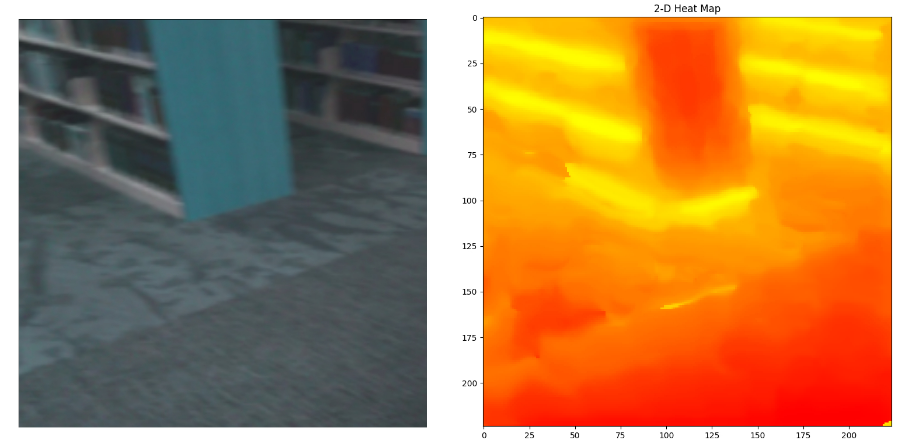
\includegraphics[width=6.5cm]{images/experiments/25.02.2022-image-pretrain-vis2.png}
    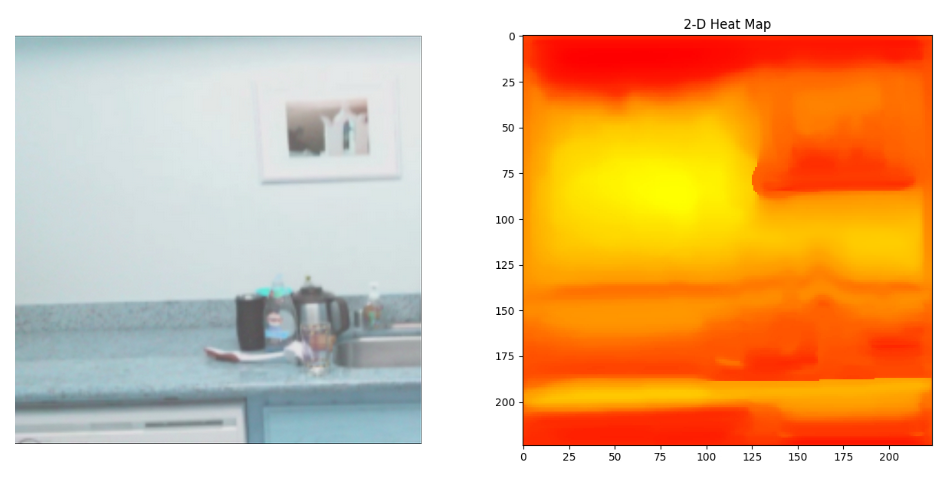
\includegraphics[width=6.5cm]{images/experiments/25.02.2022-image-pretrain-vis1.png}
    \caption{\textbf{Left} Input image. \textbf{Right} Visualization of features from the pre-trained 2D backbone}
    \label{fig:features2dvis}
\end{figure}

\begin{figure}
    \centering
    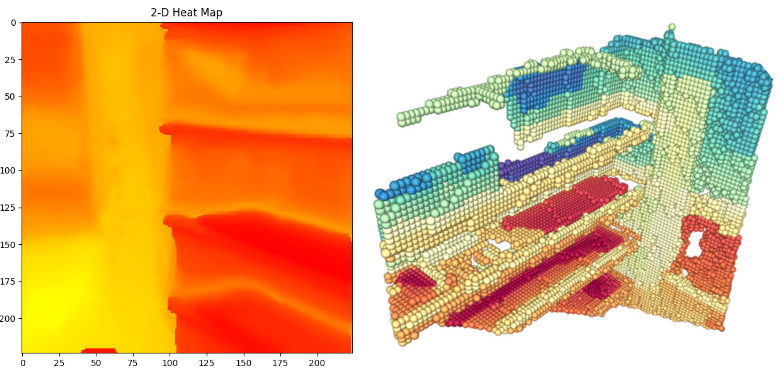
\includegraphics[width=7cm]{images/experiments/image-to-point-vis1.png}
    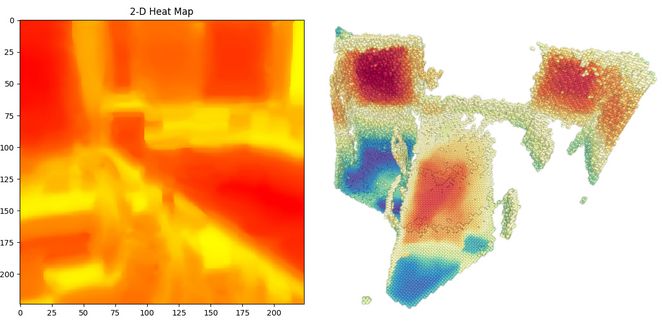
\includegraphics[width=7cm]{images/experiments/image-to-point-vis2.png}
    \caption{\textbf{Left} Visualization of transferred features on the 3D point cloud. \textbf{Right}  Visualization of features from the pre-trained 2D backbone.}
    \label{fig:features2d-3dvis}
\end{figure}

\begin{figure}
    \centering
    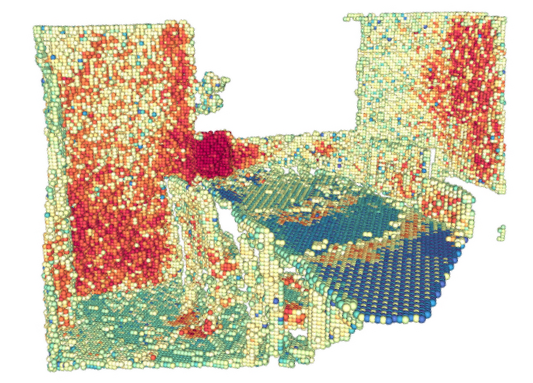
\includegraphics[width=4cm]{images/experiments/scratch-3d.png}
    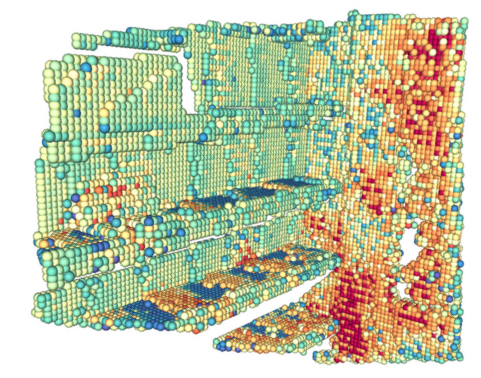
\includegraphics[width=4cm]{images/experiments/scratch-3d-2.png}
    \caption{Visualization of point features without pre-training.}
    \label{fig:features2dScratchvis}
\end{figure}

\subsection{Transfering 2D features to 3D}
\label{sec:results:2d3d}

To verify that the features were transferred correctly, we used the same visualization approach taken in section \ref{sec:results:2d} but instead applied it to points. Figure \ref{fig:features2d-3dvis} shows the relation between the 2D and 3D features. Although the features did not transfer perfectly, they did on certain key areas. For example, on the wall and table in the top image and on the bookshelves in the bottom image.

\subsection{Semantic Segmentation}
\label{sec:results:semantic}

We first test the case of pre-training our model on ScannetV2 and fine-tuning on S3DIS. Detailed results are shown in table \ref{table:s3disResults}. Fully supervised pre-training has a drastic impact on the final downstream performance ($+5.1$ mIOU) and is used as a pseudo upper bound on expected performance. Almost all base algorithms improve downstream results, except DepthContrast. Our algorithm is comparable to PointContrast, both achieving a 1\% mIOU increase but perform worse than CSC.

To simulate the use-case of capturing a large amount of un-labeled data for pre-training and only labeling a subset of it, we took Scannet and partitioned it into different portions of labeled data. The results can be found in table \ref{table:scannetVaryingDataAmount}. All methods show no improvement when given access to labels for the entire dataset. However, as the labeled data is restricted, the pre-trained models start to have an impact, with all methods improving upon training from scratch when given access to only 5\% of the labels.

Similarly, we also test varying data amounts on the semanticKITTI dataset which can be found in table \ref{table:kittiSemanticResults}. We pre-trained all methods on Scannet to see how well the learned representations transferred to different data domains. In almost all cases there are performance improvements with CSC achieving the biggest increases. Unlike in Scannet, all algorithms have some impact across all labeled data ratios. Also having more labeled data increased the performance boost of the pre-trained model, which is the opposite of what we saw in Scannet and S3DIS. This suggests that pre-training on a dataset which is out-of-distribution from the labeled dataset is more informative than pre-training on in-distribution.

\begin{table}
    \centering
    \resizebox{0.45\textwidth}{!}{
        \begin{tabular}{ c | c c c c }
                                                                & Scan & Overlap  & Semantic (mIOU)               & Instance (mAP@0.5)            \\
            \hline
            Scratch                                             & --   & --       & 65.1                          & 53.0                          \\
            Supervised                                          & --   & --       & \textbf{70.2} \textbf{(+5.1)} & \textbf{56.2} \textbf{(+3.2)} \\
            \hline
            $\dagger$ PointContrast \cite{xie2020pointcontrast} & Pair & $>$ 30\% & 66.2 \textbf{(+1.1)}          & 54.8 \textbf{(+1.8)}          \\
            PointContrast \cite{xie2020pointcontrast}           & Pair & $>$ 70\% & 68.6 \textbf{(+3.5)}          & 55.3 \textbf{(+2.3)}          \\
            PointContrast  \cite{xie2020pointcontrast}          & Same & --       & 65.0 (-0.1)                   & 56.6 \textbf{(+3.6)}          \\
            $\dagger$ CSC \cite{hou2021Exploring}               & Pair & $>$ 30\% & 69.0 \textbf{(+3.9)}          & 57.8 \textbf{(+4.8)}          \\
            CSC \cite{hou2021Exploring}                         & Pair & $>$ 70\% & \textbf{70.1} \textbf{(+5.0)} & \textbf{58.9} \textbf{(+5.9)} \\
            CSC \cite{hou2021Exploring}                         & Same & --       & 67.9 \textbf{(+2.8)}          & 57.2 \textbf{(+4.2)}          \\
            $\dagger$ DepthContrast \cite{zhang2021Self}        & Same & --       & 64.9 (-0.2)                   & 52.3 (-0.7)                   \\
            \hline
            $\dagger$ CME \textbf{(Ours)}                       & Same & --       & 66.5 \textbf{(+1.4)}          & 55.8 \textbf{(+2.8)}          \\
        \end{tabular}
    }
    \caption{\textbf{S3DIS downstream performance.} All methods use weights pre-trained on Scannet. Those with a $\dagger$ indicate the original algorithm whereas all others are variants. The difference in brackets is with respect to training from scratch.}
    \label{table:s3disResults}
\end{table}

\begin{table}
    \centering
    \resizebox{0.47\textwidth}{!}{
        \begin{tabular}{ c | c c c c c c }
                                                      & 5\%                  & 10\%                 & 20\%                  & 30\%                 & 40\%                 & 100\%                \\
            \hline
            Scratch                                   & 39.2                 & 40.4                 & 41.1                  & 41.7                 & 40.8                 & 41.0                 \\
            \hline
            PointContrast \cite{xie2020pointcontrast} & 40.3 \textbf{(1.1)}  & 42.6 \textbf{(+2.2)} & 42.2  \textbf{(+1.1)} & 41.7 \textbf{(+0.0)} & 43.0 \textbf{(+2.2)} & 42.1 \textbf{(+1.1)} \\
            CSC \cite{hou2021Exploring}               & 40.6 \textbf{(+1.4)} & 42.2 \textbf{(+1.8)} & 42.3 \textbf{(+1.2)}  & 42.2 \textbf{(+0.6)} & 44.3 \textbf{(+3.5)} & 43.0 \textbf{(+2.0)} \\
            DepthContrast \cite{zhang2021Self}        & 39.7 \textbf{(+0.5)} & 40.9 \textbf{(+0.5)} & 41.2 \textbf{(+0.1)}  & 41.9 \textbf{(+0.2)} & --                   & --                   \\
            \hline
            CME \textbf{(Ours)}                       & 39.5 \textbf{(+0.3)} & 40.9 \textbf{(+0.5)} & 40.9 (-0.2)           & 41.8 \textbf{(+0.1)} & 41.8 \textbf{(+1.0)} & 42.0 \textbf{(+1.0)} \\
        \end{tabular}
    }
    \caption{\textbf{KITTI Semantic Segmentation results (mIOU)}. All methods use weights pre-trained on Scannet. The difference in brackets is with respect to training from scratch.}
    \label{table:kittiSemanticResults}
\end{table}

\begin{table*}[ht!]
    \centering
    \resizebox{\textwidth}{!}{
        \begin{tabular}{ c | c c | c c c c c c | c c c c c c |}
                                                                &      &          & \multicolumn{6}{|c|}{Semantic Segmentation (mIOU)} & \multicolumn{6}{|c|}{Instance Segmentation (mAP@0.5)}                                                                                                                                                                                                                               \\
                                                                & Scan & Overlap  & 5\%                                                & 10\%                                                  & 20\%                 & 30\%                 & 40\%                 & 100\%                 & 5\%                  & 10\%                 & 20\%                 & 30\%                 & 40\%        & 100\%                \\
            \hline
            Scratch                                             & --   & --       & 42.2                                               & 51.1                                                  & 58.2                 & 59.2                 & 62.2                 & 67.4                  & 26.9                 & 36.3                 & 40.7                 & 42.2                 & 45.7        & 49.0                 \\
            \hline
            $\dagger$ PointContrast \cite{xie2020pointcontrast} & Pair & $>$ 30\% & 44.8 \textbf{(+2.6)}                               & 55.3 \textbf{(+4.2)}                                  & 58.0 (-0.2)          & 59.0 (-0.2)          & 63.2 \textbf{(+1.0)} & 66.9 (-0.5)           & 27.0 \textbf{(+0.1)} & 35.3 (-1.0)          & 40.5 (-0.2)          & 43.0 \textbf{(+0.8)} & 43.9 (-1.8) & 49.1 \textbf{(+0.1)} \\
            PointContrast \cite{xie2020pointcontrast}           & Pair & $>$ 70\% & 46.1 \textbf{(+3.9)}                               & 50.7 (-0.4)                                           & 58.0 (-0.2)          & 61.9 \textbf{(+2.7)} & 62.6 \textbf{(+0.4)} & 67.3 (-0.1)           & 28.0 \textbf{(+1.1)} & 35.7 (-0.6)          & 40.5 (-0.2)          & 42.8 \textbf{(+0.6)} & 44.4 (-1.3) & --                   \\
            PointContrast \cite{xie2020pointcontrast}           & Same & --       & 45.5 \textbf{(+3.3)}                               & 48.8 (-2.3)                                           & 56.7 (-1.5)          & 59.3 \textbf{(+0.1)} & 61.7 (-0.5)          & 66.5 (-0.9)           & --                   & --                   & --                   & --                   & --          & --                   \\
            $\dagger$ CSC \cite{hou2021Exploring}               & Pair & $>$ 30\% & 42.6 \textbf{(+0.4)}                               & 53.0 \textbf{(+1.9)}                                  & 57.3 (-0.9)          & 62.2 \textbf{(+3.0)} & 65.2 \textbf{(+3.0)} & 67.6 \textbf{(+0.2)}  & 29.8 \textbf{(+2.9)} & 35.5 (-0.8)          & 41.6 \textbf{(+0.9)} & 42.9 \textbf{(+0.7)} & 44.6 (-1.1) & 49.3 \textbf{(+0.3)} \\
            CSC \cite{hou2021Exploring}                         & Pair & $>$ 70\% & 45.4 \textbf{(+3.2)}                               & 50.8 (-0.3)                                           & 59.3 \textbf{(+1.1)} & 59.7 \textbf{(+0.5)} & 62.7 \textbf{(+0.5)} & 68.0 \textbf{(+0.6)}  & 29.8 \textbf{(+2.9)} & 37.6 \textbf{(+1.3)} & 41.4 \textbf{(+0.7)} & --                   & --          & --                   \\
            CSC \cite{hou2021Exploring}                         & Same & --       & 44.1 \textbf{(+1.9)}                               & 50.9 (-0.2)                                           & 56.6 (-1.6)          & 58.9 (-0.3)          & 61.5 (-0.7)          & 67.4 \textbf{(+0.0)}  & 28.8 \textbf{(+1.9)} & 37.2 \textbf{(+0.9)} & 42.0 \textbf{(+1.3)} & --                   & --          & --                   \\
            $\dagger$ DepthContrast \cite{zhang2021Self}        & Same & --       & 49.3 \textbf{(+7.1)}                               & 54.3 \textbf{(+3.2)}                                  & 58.2 \textbf{(+0.0)} & 59.6 \textbf{(+0.4)} & 63.2 \textbf{(+1.0)} & 67.4 \textbf{(+0.0)}  & 24.9 (-2.0)          & 33.8 (-2.5)          & 38.2 (-2.5)          & 42.0 (-0.2)          & 42.0 (-3.7) & 48.7 (-0.3)          \\
            \hline
            $\dagger$ CME \textbf{(Ours)}                       & Same & --       & 44.0 \textbf{(+1.8)}                               & 53.0 \textbf{(+1.9)}                                  & 58.6 \textbf{(+0.4)} & 60.7 \textbf{(+1.5)} & 63.3 \textbf{(+1.1)} & 67.7 \textbf{(+0.28)} & 25.5 (-1.4)          & 35.5 (-0.8)          & 39.1 (-1.6)          & 42.4 \textbf{(+0.2)} & 43.6 (-2.1) & 48.5 (-0.5)          \\
        \end{tabular}
    }
    \caption{\textbf{Scannet downstream performance.} All methods use weights pre-trained on Scannet. Those with a † indicate the original algorithm whereas all others are variants. The difference in brackets is with respect to training from scratch. }
    \label{table:scannetVaryingDataAmount}
\end{table*}

\subsection{Instance Segmentation}
\label{sec:results:instance}

As in the previous section, we evaluate the performance of pre-training on Scannet and training on S3DIS for instance segmentation which can be found in table \ref{table:s3disResults}. Almost all pre-training methods get close or even surpass supervised results with the exception again being DepthContrast. The best performing method, as before, is Contrastive Scene Contexts which gets a performance boost of 4.8 mAP@0.5. However, our own method gets very close to supervised level performance with a boost of 2.8.

However, looking at the effects on Scannet in table \ref{table:scannetVaryingDataAmount}, all methods struggle to improve upon training from scratch. In many cases they even perform substantially worse, with out method not being able to improve in almost all scenarios. Contrastive Scene Contexts is the only method that shows some consistent improvement. It is interesting to note that even though semantic segmentation receives a boost, this does not necessarily translate into instance segmentation.

\subsection{Object Detection}
\label{sec:results:object}

Object detection is an interesting downstream task because it operates at an object level instead of a point level like the pre-training objective. Here we investigated the performance on Scannet and SunRGBD, which can be found in table \ref{table:scannetObjectDetection}.

All methods besides DepthContrast show a strong improvement in both datasets. Contrastive Scene Contexts perform get the largest boost on SunRGBD of 3.1 mAP while our method gets the largest boost on Scannet with an increase of 2.5 mAP. All methods are still pre-trained on Scannet only and so to see performance improvements when using the entire Scannet dataset indicated that in the case of object detection, pre-training can help even on larger datasets.


\begin{table}
    \centering
    \resizebox{0.3\textwidth}{!}{
        \begin{tabular}{c | c c c}
                                & Scannet              & SunRGBD              \\
            \hline
            Scratch             & 35.2                 & 32.0                 \\
            \hline
            PointContrast       & 36.7 \textbf{(+1.5)} & 34.2 \textbf{(+2.2)} \\
            CSC                 & 36.1 \textbf{(+0.9)} & 35.1 \textbf{(+3.1)} \\
            DepthContrast       & 33.9 (-1.3)          & 32.9 \textbf{(+0.9)} \\
            \hline
            CME \textbf{(Ours)} & 37.7 \textbf{(+2.5)} & 33.1 \textbf{(+1.1)} \\
        \end{tabular}
    }
    \caption{\textbf{Object Detection using VoteNet (mAP)}}
    \label{table:scannetObjectDetection}
\end{table}

\section{Analysis}
\label{sec:analysis}

\subsection{Varying Overlap}
\label{sec:results:varying}

\subsection{Training Speedup}
\label{sec:results:speedup}

Talk about graphs showing that you can get close to final performance within a fraction of the time.

\subsection{Inconsistencies in Performance Boost}
\label{sec:results:inconsistencies}

When using point correspondences without overlapping scans, the performance gain disappears almost entirely. This was noted in their original work and suggests to us that it is learning better features only due to its ability to better extrapolate surfaces.

Our algorithm is the only one that shows a consistent increase across varying Scannet data portions as well as S3DIS. Unlike PointContrast and CSC, our algorithm does not require pose transformations between adjacent scans making it easier to implement.

The performance gains are unpredictable as the fraction of labeled data is varied. A performance boost of 3\% at 30\% labeled data can turn into a performance drop at 20\% labeled data. At the extreme of using 5\% labeled data, all algorithms have a performance boost. This further reinforces the idea that pre-training is most useful when the amount of labeled data is extremely limited. Interestingly, DepthContrast which was the worst performing on S3DIS is the best performing by a large margin on Scannet at 5\% labeled data, again showing the unpredictability of the results.

\section{Conclusion}
\label{sec:conclusion}

\begin{itemize}
    \item that transferring 2D features to 3D improves performance across different domains.
    \item that although some algorithms perform extremely well in some domains, they fail in others. Or they might work well on one task but not another.
    \item PointContrast \& CSC both ideally require overlapping scenes to perform properly whereas our algorithm does not.
    \item Pre-training does little when large labeled datasets are used but are more effective when datasets are very small
    \item Pre-training can help speed up training time on smaller datasets but has no impact on larger datasets.
    \item Overal can expect about a 1\% increase in performance
    \item Our method, which is easy to implement and does not require a pose transformation between frames, is a good start in trying to find best performance.
    \item Also when using PointContrast \& CSC, you can experiment with overlap ratio and using tha same scan to get better results
    \item It may be worth trying a self-supervised method to see performance boost before spending extra time labeling the entire dataset
    \item Using out-of-distribution data for pre-training can have a bigger impact that pre-training on in-distribution.
\end{itemize}

\begin{figure}[h!]
    \centering
    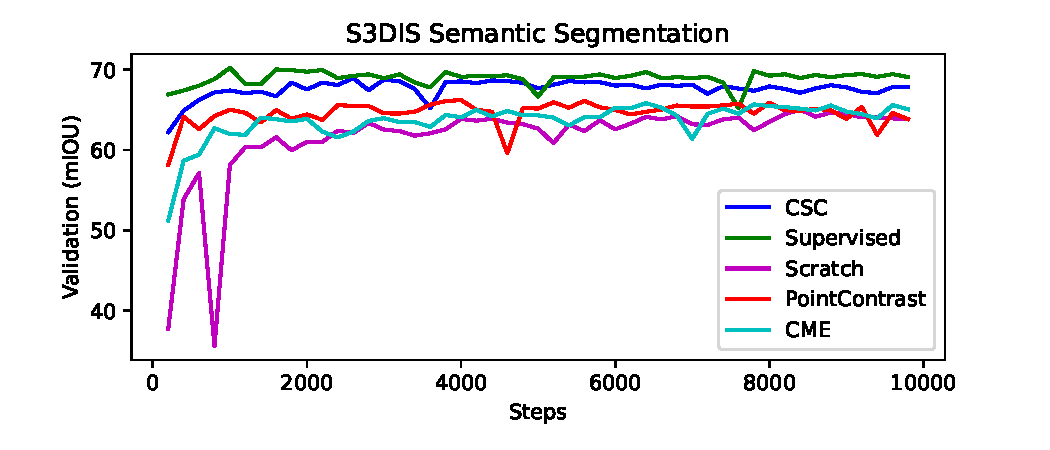
\includegraphics[width=8cm]{images/plots/s3dis_semantic.pdf}
    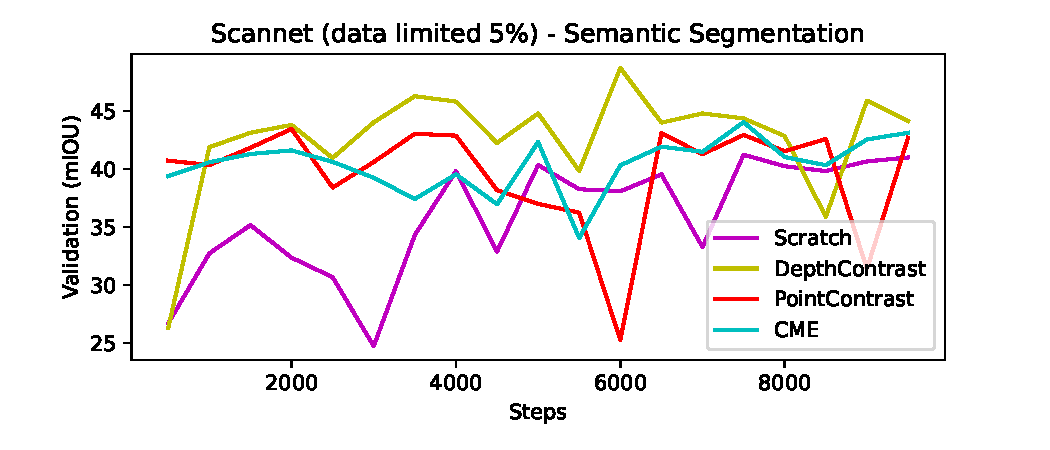
\includegraphics[width=8cm]{images/plots/scannet_0.05_semantic.pdf}
    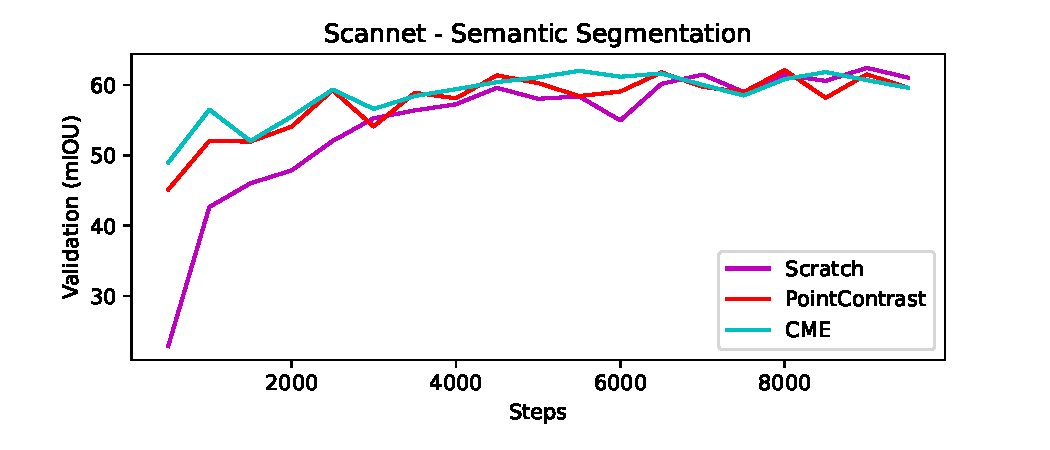
\includegraphics[width=8cm]{images/plots/scannet_semantic.pdf}
    \caption{Comparison of validation performance over training steps for models pre-trained on Scannet and fine-tuned for semantic segmentation on: \textbf{Top:} S3DIS, \textbf{Middle:} Scannet with only 5\% labeled data, \textbf{Bottom:} Scannet}
    \label{fig:validationComparison}
\end{figure}


\clearpage
%%%%%%%%% REFERENCES
{\small
    \bibliographystyle{ieee_fullname}
    \bibliography{paper}
}

\clearpage
\section{Supplement}

\begin{table*}[t!]
    \centering
    \resizebox{\textwidth}{!}{
        \begin{tabular}{ c | c c c c c c c c c c c c c | c }
                                                      & ceiling        & floor          & wall           & beam           & column         & window         & door           & table          & chair          & sofa           & bookcase       & board          & clutter        & mIOU                            \\
            \hline
            Scratch                                   & 90.34          & \textbf{96.84} & 80.63          & 0              & 25.5           & 56.95          & 62.93          & 75.14          & 86.21          & 65.77          & 72.12          & 76.91          & 56.4           & 65.06                           \\
            Supervised                                & \textbf{91.81} & 96.74          & \textbf{84.11} & \textbf{0.21}  & \textbf{34.68} & \textbf{57.64} & \textbf{81.53} & \textbf{77.63} & \textbf{89.82} & \textbf{85.76} & \textbf{76.03} & \textbf{79.27} & \textbf{57.67} & \textbf{70.22} \textbf{(+5.16)} \\
            \hline
            PointContrast                             & 91.97          & \textbf{96.67} & 82.4           & 0              & 17.84          & 56.49          & \textbf{75.39} & \textbf{77.63} & 87.35          & 63.3           & 73.53          & \textbf{79.55} & 58.76          & 66.22 \textbf{(+1.16)}          \\
            PointContrast - Same Scan                 & 91.03          & 96.27          & \textbf{82.8}  & 0              & 31.53          & 57.27          & 69.33          & 76.97          & \textbf{88.83} & 45.49          & 71.02          & 77.09          & 57.06          & 64.97 (-0.09)                   \\
            PointContrast - 70\% overlap              & 91.85          & 96.56          & 83.55          & 0              & 28.25          & 59.36          & 73.53          & 78.51          & 88.28          & 79.95          & 74.61          & 76             & 61.08          & 68.58 \textbf{(+3.52)}          \\
            Contrastive Scene Contexts                & \textbf{92.34} & 96.02          & 83.53          & 0              & \textbf{40.88} & \textbf{57.73} & 72.11          & 77.5           & 88.15          & \textbf{74.61} & \textbf{74.52} & 76.45          & \textbf{62.64} & 68.96 \textbf{(+3.9)}           \\
            Contrastive Scene Contexts - Same Scan    & 91.68          & 96.59          & 83.21          & 0              & 40.38          & 58.12          & 70.42          & 76.77          & 87.13          & 69.33          & 68.77          & 82.34          & 58.45          & 67.94 \textbf{(+2.88)}          \\
            Contrastive Scene Contexts - 70\% overlap & 92.68          & 96.63          & 83.99          & 0              & 42.37          & 55.95          & 77.17          & 75.74          & 89.57          & 82.74          & 73.45          & 80.67          & 60.55          & \textbf{70.12} \textbf{(+5.06)} \\
            DepthContrast                             & 90.99          & 95.45          & 80.99          & 0              & 32.52          & 51.94          & 61.57          & 74.55          & 87.28          & 71.62          & 71.34          & 67.71          & 57.85          & 64.91 (-0.15)                   \\
            CME \textbf{(Ours)}                       & 90.8           & 96.57          & 82.52          & \textbf{0.110} & 30.94          & 56.94          & 68.71          & 75.12          & 88.48          & 71.7           & 72.17          & 73.783         & 56.35          & 66.48 \textbf{(+1.42)}          \\
        \end{tabular}
    }
    \caption{S3DIS Semantic Segmentation results (mIOU)}
\end{table*}

\begin{table*}[t!]
    \centering
    \resizebox{0.8\textwidth}{!}{
        \begin{tabular}{ c | c c c c c c c c c c | c }
                                                      & beam & column        & window        & door & table         & chair         & sofa          & bookcase      & board         & clutter       & mAP@0.5                       \\
            \hline
            Scratch                                   & 0    & 12.8          & 61.7          & 92.0 & 51.4          & 87.3          & 62.4          & 38.5          & 87.0          & 37.1          & 53.0                          \\
            Supervised                                & 0    & 26.0          & 74.3          & 84.5 & 43.3          & 87.3          & \textbf{81.8} & 37.4          & \textbf{85.4} & \textbf{41.2} & \textbf{56.2} (+3.2)          \\
            \hline
            PointContrast                             & 0    & 24.7          & 67.9          & 90.7 & 43.8          & 92.0          & 72.7          & 32.3          & 85.6          & 38.0          & 54.8 \textbf{(+1.8)}          \\
            PointContrast - Same Scan                 & 0    & 19.8          & 70.7          & 92.1 & 48.4          & 90.5          & 81.8          & 38.4          & 90.4          & 34.1          & 56.6 \textbf{(+3.6)}          \\
            PointContrast - 70\% overlap              & 0    & 22.6          & 71.6          & 94.6 & 45.8          & 87.9          & 71.7          & 37.0          & 81.0          & 40.9          & 55.3 \textbf{(+2.3)}          \\
            Contrastive Scene Contexts                & 0    & 32.9          & 69.2          & 93.0 & 47.6          & 87.5          & 80.9          & 39.6          & 87.5          & 40.4          & 57.8 \textbf{(+4.8)}          \\
            Contrastive Scene Contexts - Same Scan    & 0    & 32.0          & 69.3          & 96.1 & 38.7          & 89.4          & 87.6          & 38.8          & 81.3          & 38.8          & 57.2 \textbf{(+4.2)}          \\
            Contrastive Scene Contexts - 70\% overlap & 0    & 27.2          & 76.9          & 95.4 & 42.2          & 90.3          & 90.9          & 42.6          & 84.7          & 38.7          & \textbf{58.9} \textbf{(+5.9)} \\
            DepthContrast                             & 0    & 40.3          & 68.4          & 74.9 & 42.2          & 87.8          & 62.4          & 33.3          & 78.1          & 35.5          & 52.3 (-0.7)                   \\
            CME \textbf{(Ours)}                       & 0    & \textbf{35.0} & \textbf{70.0} & 83.4 & \textbf{53.9} & \textbf{88.9} & 71.7          & \textbf{42.2} & 76.1          & 36.7          & 55.8 \textbf{(+2.8)}          \\
        \end{tabular}
    }
    \caption{S3DIS Instance Segmentation Results (mAP@0.5)}
\end{table*}

\begin{table*}[t!]
    \centering
    \resizebox{0.8\textwidth}{!}{
        \begin{tabular}{ c | c c c c c c}
                                                      & 5\%                    & 10\%                   & 20\%                   & 30\%                   & 40\%                   & 100\%                  \\
            \hline
            Scratch                                   & 42.2                   & 51.09                  & 58.23                  & 59.23                  & 62.17                  & 67.43                  \\
            \hline
            PointContrast                             & 44.79 \textbf{(+2.59)} & 55.28 \textbf{(+4.19)} & 57.98 (-0.25)          & 58.97 (-0.26)          & 63.17 \textbf{(+1.00)} & 66.88 (-0.55)          \\
            Contrastive Scene Contexts                & 42.6 \textbf{(+0.4)}   & 53.03 \textbf{(+1.94)} & 57.28 (-0.95)          & 62.15 \textbf{(+2.92)} & 65.15 \textbf{(+2.98)} & 67.62 \textbf{(+0.19)} \\
            Contrastive Scene Contexts - 70\% overlap & 45.44 \textbf{(+3.24)} & 50.84 (-0.25)          & 59.26 \textbf{(+1.03)} & 59.72 \textbf{(+0.49)} & 62.72 \textbf{(+0.55)} & 68.01 \textbf{(+0.58)} \\
            Contrastive Scene Contexts - same scan    & 44.09 \textbf{(+1.89)} & 50.88 (-0.21)          & 56.64 (-1.59)          & 58.9 (-0.33)           & 61.50 (-0.67)          & 67.37 (-0.06)          \\
            CME \textbf{(Ours)}                       & 44.04 \textbf{(+1.84)} & 52.97 \textbf{(+1.88)} & 58.6 \textbf{(+0.37)}  & 60.73 \textbf{(+1.5)}  & 63.31 \textbf{(+1.14)} & 67.71 \textbf{(+0.28)} \\
        \end{tabular}
    }
    \caption{Scannet Semantic Segmentation with Partial Data  (mIOU)}
\end{table*}

\begin{table*}[t!]
    \centering
    \resizebox{0.7\textwidth}{!}{
        \begin{tabular}{ c | c c c c c c}
                                       & 5\%                  & 10\%          & 20\%                 & 30\%                 & 40\%        & 100\%                \\
            \hline
            Scratch                    & 26.9                 & \textbf{31.1} & 40.7                 & 42.2                 & 45.7        & 49.0                 \\
            \hline
            PointContrast              & 27.0 \textbf{(+0.1)} & 35.3          & 40.5 (-0.2)          & 43.0 \textbf{(+0.8)} & 43.9 (-1.8) & 49.1 \textbf{(+0.1)} \\
            Contrastive Scene Contexts & 29.8 \textbf{(+2.9)} & 35.5          & 41.6 \textbf{(+0.9)} & 42.9 \textbf{(+0.7)} & 44.6 (-1.1) & 49.3 \textbf{(+0.3)} \\
            CME \textbf{(Ours)}        & 25.5 (-1.4)          & 35.5          & 39.1 (-1.6)          & 42.4 \textbf{(+0.2)} & 43.6 (-2.1) & 48.5 (-0.5)          \\
        \end{tabular}
    }
    \caption{Scannet Instance Segmentation with Partial Data  (mAP@0.5)}
\end{table*}

\begin{table*}[t!]
    \centering
    \resizebox{0.7\textwidth}{!}{
        \begin{tabular}{ c | c c c c c c }
                                       & 5\%                    & 10\%                   & 20\%                   & 30\%                   & 40\%                   & 100\%                  \\
            \hline
            Scratch                    & 39.2                   & 40.43                  & 41.06                  & 41.67                  & 40.79                  & 41.01                  \\
            \hline
            PointContrast              & 40.29 \textbf{(1.09)}  & 42.59 \textbf{(+2.16)} & 42.2  \textbf{(+1.14)} & 41.65 (-0.02)          & 42.99 \textbf{(+2.2)}  & 42.09 \textbf{(+1.08)} \\
            Contrastive Scene Contexts & 40.6 \textbf{(+1.4)}   & 42.21 \textbf{(+1.78)} & 42.26 \textbf{(+1.2)}  & 42.24 \textbf{(+0.57)} & 44.29 \textbf{(+3.5)}  & 43.01 \textbf{(+2.0)}  \\
            CME \textbf{(Ours)}        & 39.49 \textbf{(+0.29)} & 40.90 \textbf{(+0.47)} & 40.91 (-0.15)          & 41.82 \textbf{(+0.15)} & 41.77 \textbf{(+0.98)} & 42.04 \textbf{(+1.03)} \\
        \end{tabular}
    }
    \caption{KITTI Semantic Segmentation results (mIOU)}
\end{table*}

\begin{table*}[t!]
    \centering
    \resizebox{0.4\textwidth}{!}{
        \begin{tabular}{c | c c c}
                                       & Scannet              & SunRGBD              \\
            \hline
            Scratch                    & 35.2                 & 32.0                 \\
            \hline
            PointContrast              & 36.7 \textbf{(+1.5)} & 34.2 \textbf{(+2.2)} \\
            Contrastive Scene Contexts & 36.1 \textbf{(+0.9)} & 35.1 \textbf{(+3.1)} \\
            DepthContrast              & 33.9 (-1.3)          &                      \\
            CME \textbf{(Ours)}        & 37.7 \textbf{(+2.5)} & 33.1 \textbf{(+1.1)} \\
        \end{tabular}
    }
    \caption{Object Detection using VoteNet  (mAP)}
\end{table*}

\end{document}